\documentclass[american]{rtxreport}

\usepackage{listings}
\usepackage[utf8]{inputenc}

\author{David Pineau}
\title{Technical Documentation}

\rtxdoctype{Technical Documentation}
\rtxdocref{technical\_documentation}
\rtxdocversion{0.7}
\rtxdocstatus{Release}

\rtxdochistory{
0.1 & 10/03/2011 & David Pineau & Plan of the Technical Documentation \\
\hline
0.2 & 11/03/2011 & David Pineau & Chapters 1 to 3 done Intro and Chapter
                                  4 still missing \\
\hline
0.3 & 11/03/2011 & Louis Opter & Cosmetic improvements \\
\hline
0.4 & 13/08/2011 & David Pineau & Added cache description section to chapter 4\\
\hline
0.5 & 13/08/2011 & David Pineau & Added compilation steps sections to chapter 4\\
\hline
0.6 & 01/09/2011 & David Pineau & Finished template compilation steps in the chapter 4\\
\hline
0.7 & 11/09/2011 & Louis Opter & Minor improvements in ``Template Compilation'' \\
\hline
0.6 & 04/01/2012 & David Pineau & Adding of the front compilation process + update of backend compilation process \\
}

\newcommand{\note}[1]{\marginpar{\scriptsize{\textdagger\ #1}}}



\definecolor{lstbackground}{rgb}{0.95, 0.95, 0.95}
\definecolor{lstcomment}{rgb}{0, 0.12, 0.76}
\definecolor{lstkeyword}{rgb}{0.66, 0.13, 0.78}
\definecolor{lststring}{rgb}{0.67, 0.7, 0.13}
\definecolor{lstidentifier}{rgb}{0.1, 0.1, 0.1}

\lstset{
        tabsize=2,
        captionpos=b,
        emptylines=1,
        frame=single,
        breaklines=true,
        extendedchars=true,
        showstringspaces=false,
        showspaces=false,
        showtabs=false,
        basicstyle=\color{black}\small\ttfamily,
        numberstyle=\scriptsize\ttfamily,
        keywordstyle=\color{lstkeyword},
        commentstyle=\color{lstcomment},
        identifierstyle=\color{lstidentifier},
        stringstyle=\color{lststring},
        backgroundcolor=\color{lstbackground}
}

\definecolor{grey}{rgb}{0.90,0.90,0.90}
\definecolor{rBlue}{rgb}{0.0,0.24,0.96}
\definecolor{rRed}{rgb}{0.6,0.0,0.0}
\definecolor{rGreen}{rgb}{0.0,0.4,0.0}

\lstdefinelanguage{rtx}%
{
	morekeywords={DECLARE, SEQUENCE, INTERFACE, IMPLEMENTATION, FROM, READ,
        OPTIONAL, CONFIGURATION_VARIABLE, USE, AS, WITH, SEQUENCES, ON, ELSE,
        LET, PROVIDES, REQUIRE, THROWS, FINALLY, FOREACH, IN, AND, OR, THROW,
        HANDLE_ERROR, NOT, REGISTER, LIKE, BIT, INTEGER, DOUBLE, BOOLEAN,
        STRING, MAPPED_AT, PCI},%
	sensitive=true,%
	morecomment=[l][\color{rRed}]{//},%
 	morecomment=[l][\color{rRed}]{\#},%
	morecomment=[s][\color{rRed}]{/*}{*/},%
	morestring=[b][\color{rGreen}]",%
	morestring=[b][\color{rGreen}]',%
	keywordstyle={\color{rBlue}}%
}[keywords,comments,strings]

\lstdefinelanguage{rti}%
{
	morekeywords={interface,
        builtin,
        type, sequence, variable,
        provided, required, optional},%
	sensitive=true,%
	morecomment=[l][\color{rRed}]{//},%
 	morecomment=[l][\color{rRed}]{\#},%
	morecomment=[s][\color{rRed}]{/*}{*/},%
	morestring=[b][\color{rGreen}]",%
	morestring=[b][\color{rGreen}]',%
	keywordstyle={\color{rBlue}}%
}[keywords,comments,strings]

\lstdefinelanguage{blt}%
{
	morekeywords={template,
        decl, stmt},%
	sensitive=true,%
	morecomment=[l][\color{rRed}]{//},%
 	morecomment=[l][\color{rRed}]{\#},%
	morecomment=[s][\color{rRed}]{/*}{*/},%
	morestring=[b][\color{rGreen}]",%
	morestring=[b][\color{rGreen}]',%
	keywordstyle={\color{rBlue}}%
}[keywords,comments,strings]





\begin{document}

\maketitle

\rtxmaketitleblock

\tableofcontents

\begin{abstract}
    This document describes how the \rtx\ compiler works, starting with the
    different steps of the compilation process, up to how it is implemented.
\end{abstract}


%\section*{Introduction}
%% What is Rathaxes
%% What is this document about exactly



\chapter{The tools that constitute \rtx}

\section{The language: CodeWorker}

\emph{CodeWorker} is an Open Source parsing tool and a source code generator
devoted to generative programming made by Cédric Lemaire. Generative
programming is a software engineering approach interested in automating the
production of reusable, tailor-made, adaptable and reliable IT systems. In
layman's terms, \emph{CodeWorker} lets you generate code by parsing existing
languages, or by creating and parsing your own language. We will be using it
for this exact purpose as ``a compiler of compilers''. Once a language file has
been parsed, CodeWorker provides several techniques for generating code.

The tool's scripting language drives the parsing and source code generation
process. Its syntax is derived from the C family of languages, making it
familiar to most programmers. The template syntax is like JSP, ASP, or
Velocity. It has variations for parsing, code generation, or procedural
programming, giving the developer a number of options for organizing
\emph{CodeWorker} projects. 

\emph{Codeworker} is more powerful and easier to use than \emph{Lex/Yacc},
\emph{CodeWorker} perfectly fits \rtx' code generation needs. It can be
divided into three major parts:

\begin{itemize}
    \item \emph{BNF} description language: \emph{Codeworker}'s parsing language
        requires a simple \emph{BNF} description of the language to parse, and
        each \emph{BNF} Rule is overloadable for extension purposes. The DSL of
        \rtx\ will be described thus.
    \item Scripting language: Codeworker scripts are
        powerful enough for the tree decoration needs of \rtx.
    \item Generation scripting language: We will then use the templating
        functionalities of CodeWorker to generate C code.
\end{itemize}



\section{The CNorm library}

\emph{CNorm} is a C parsing tool written with \emph{CodeWorker} made by Lionel
Auroux (Epita/Epitech system \& security laboratory's director), Cédric Lemaire
(CodeWorker's author and developer) and David Giron, David Amsallem and
Christophe Fajardo (all from the 2009 \rtx\ team). It also contains

This parser has been designed to be as powerful as possible to be able to
parse any dialect of C (extensions with specific qualifiers and specifiers).

\begin{itemize}
    \item Standard C 89 syntax
    \item GnuC asm expressions
    \item GnuC \texttt{\_\_thread} storage class specifier
    \item GnuC parameter forward declaration
    \item GnuC \texttt{\_\_extension\_\_} avoids warnings on GnuC extensions
    \item GnuC subscript
    \item GnuC designated initializer
    \item GnuC \texttt{\_\_builtin\_offsetof}
    \item GnuC \texttt{\_\_builtin\_va\_list}
    \item c99 \texttt{static} in direct absolute declarator
    \item c99 block as single expression (\texttt{\{ \}})
    \item c99 \texttt{typeof}
    \item c99 designation
    \item c99 \texttt{\_\_alignof}
    \item c99 \texttt{complex}, \texttt{\_\_real} \& \texttt{\_\_imag operator}
    \item c99 range expression
    \item c99 and Windows attributes
    \item K. \& R. coding style
    \item Missing type in function declaration
\end{itemize}

This grammar was adapted from the one in section A13 of the C programming
language, second edition, by Brian W. Kernighan and Dennis M. Ritchie
(Englewood Cliffs, New Jersey: Prentice Hall PTR, 1988; ISBN 0-13-110362-8),
pages 234 - 238. 

Cnorm is used in \rtx\ to parse the C code present in the BDSL in order to
avoid opaque datas and to provide full control on the handled code. It is also
used for the final C driver code generation. The C abstract syntax tree
organisation ca be found in Cnorm's own documentation. It won't be covered by
this one.



\chapter{Use cases of the compiler}

\section{Who will use \rtx}

As described in the Introduction, \rtx\ is aimed at two kinds of developers.

The primary target is the device driver developer. He will write a code
describing the algorithms to implement for the specific device he's writing
the driver for.

The secondary target is the kernel developer. His role is to implement the
template library that contains a templated C code containing the
OS-specific code.

Finally, a third kind of developer will have yet another role in the
development of a device driver. Using a ``State Of the Art'' of writing a
driver, he will design an interface that both the kernel developer and
the device driver developer will have to follow in their codes.

\section{The three parts of the DSL}

As you can see, three kinds of users and developers will interact with \rtx,
and make it evolve, each focused on a specific part of the DSL.
Each one of those three parts has its own place and function in the process of
compiling a \rtx\ driver.

\subsection{\rtx\ Maintainer: the Middle-End}
\lstset{language=rti}

First and foremost, although not really the first visible kind of contributor
to the language, is the \rtx\ maintainer. As described earlier, his role is
to design an interface that will have to be respected by both of the other kinds
of developer that will use our compiler and code in \rtx.

Those interfaces are part of what we will now call the \emph{Middle-End} of the
language. It could be seen as an compiler-internal description of what is
required or optional for both the driver's code and the template code
implementation. That will be the link between the \emph{Front-End} and the
\emph{Back-End}, by defining the available types, sequences and variables.

The file extension for this part of the DSL is \texttt{.rti} (\rtx\ Interface).

It is identified by an unique name in the compiler, generally identifying the
kind of sub-system it is created to describe.

It contains:
\begin{itemize}
    \item The types that are used in the sub-system, that must be provided by
        the template C code;
    \item The sequences (functions or algorithms) that are provided by the
        template C code;
    \item The sequences (functions or algorithms) that are required
        (they can be optional) from the device's \rtx\ driver;
    \item The configuration variables/values needed by the interface.
\end{itemize}

For example, we could have:
\begin{itemize}
    \item Userland interface: describes the \emph{LKM}'s functions and types;
    \item PCI interface: describes the PCI BUS function's and types;
    \item IO interface: describing the functions that can be used
for a device driver which device is on the IO port.
\end{itemize}

Here is an example of what an interface can look like:
\begin{lstlisting}
    interface Userland
    {
        // Here a list of compiler-builtin types
        builtin type bit;
        builtin type byte;
        builtin type word;
        builtin type dword;
        builtin type qword;

        builtin type register;
        builtin type buffer;
        builtin type context;

        // Here a type that has to be implemented in the templates
        type device;

        // Here is a sequence provided by the templates
        provided sequence concat(register, buffer);

        // Here are the sequences asked from the .rtx file
        required sequence doSomething(context, register);
        optional sequence doNothing(device);

        // Here the variables required from the .rtx file
        required variable os;
        required variable version_major;
        optional variable version_minor;
    };
\end{lstlisting}

Actually, this part of the DSL is the only one that doesn't need anything else
apart its dependencies to be checked as a valid code. In fact it is this part
that defines any generic type to be used in any other \rtx\ code.

\subsection{Kernel Developer: the Back-End}
\lstset{language=blt}

Secondly, another unavoidable kind of contributor to \rtx\ is the Kernel
Developer. This is them who will implement the backend library in order to add
the support of a new Operating System in \rtx.

The role of the \emph{Back-End} is to provide the platform-specific code for
each part of the \rtx\ (and then final) driver. The file extension is
\texttt{.blt} (\emph{Back-End} Library Template).

By using the interfaces present in itself, the compiler will be able to tell
what is supported or not for a specific Operating System, as well as telling
whether the types are used wrongly or not in the template code.

The template code is contained in a \emph{with} block that associates the code
with specific configuration variables and values. This means that the template
will be used when those specific variables equal the associated values.

Inside the \emph{with} block can be found one or more templates of code. A
template of code is identified by its type. This is the part that allows
referencing or using templates from inside others.

The content of the template is actually some instrumentalized C code that may
(or may not) be platform-dependant. By instrumented is meant that a
\rtx-specific syntax extends the C in order to use \rtx\ template
variables inside the C. This syntax also allows the concatenation of strings
in order to craft identifiers.

Here is a little example of what it can look like:
\begin{lstlisting}
    with os=Linux, version >= 2.6, bus=ioport
    {
        template get(register reg) decl
        {
            ${register} get_reg_${reg.name}(void)
            {
                return in${reg.basetype.initial}(${reg.addr});
            }
        }

        template get(register reg) stmt
        {
            get_reg_${reg.name}()
        }
    }
\end{lstlisting}

\subsection{Device driver Developer: the Front-End}
\lstset{language=rtx}

Finally, the last and most obvious part of the DSL, the so-called
\emph{Front-End}. This is the part an electronics engineer or a driver
developer will use. This part of the language possesses a syntax that allows
describing the registers of a device, how to access them, how to manipulate
them, as well as describing the algorithms that will use the device. The file
extension used for this part of the language is \texttt{.rtx} (\rtx).

One of the most important aspects of the \emph{Front-End} is that it contains a
\emph{configuration} block. This block contains the declaration of what was
earlier called the configuration variables. Those variable alter the compilation
process of a driver.

Compiling a \texttt{.rtx} file means checking the types and the availability of
each type or sequence by checking each of them against the matching interfaces
from the \emph{Middle-End}. See section
\ref{sec:driverCompilation}



\chapter{Compiler Architecture} %% take the tex code out of the AA2 doc.

\section{The different modules of the compiler}

A compiler is never a simple program. In the case of \rtx, we can identify
different elements inside the core of the compiler. Since the flexibility and
scalability of the language is one of the side-goals of the project,
those modules were an absolute necessity. Here is the diagram showing them:

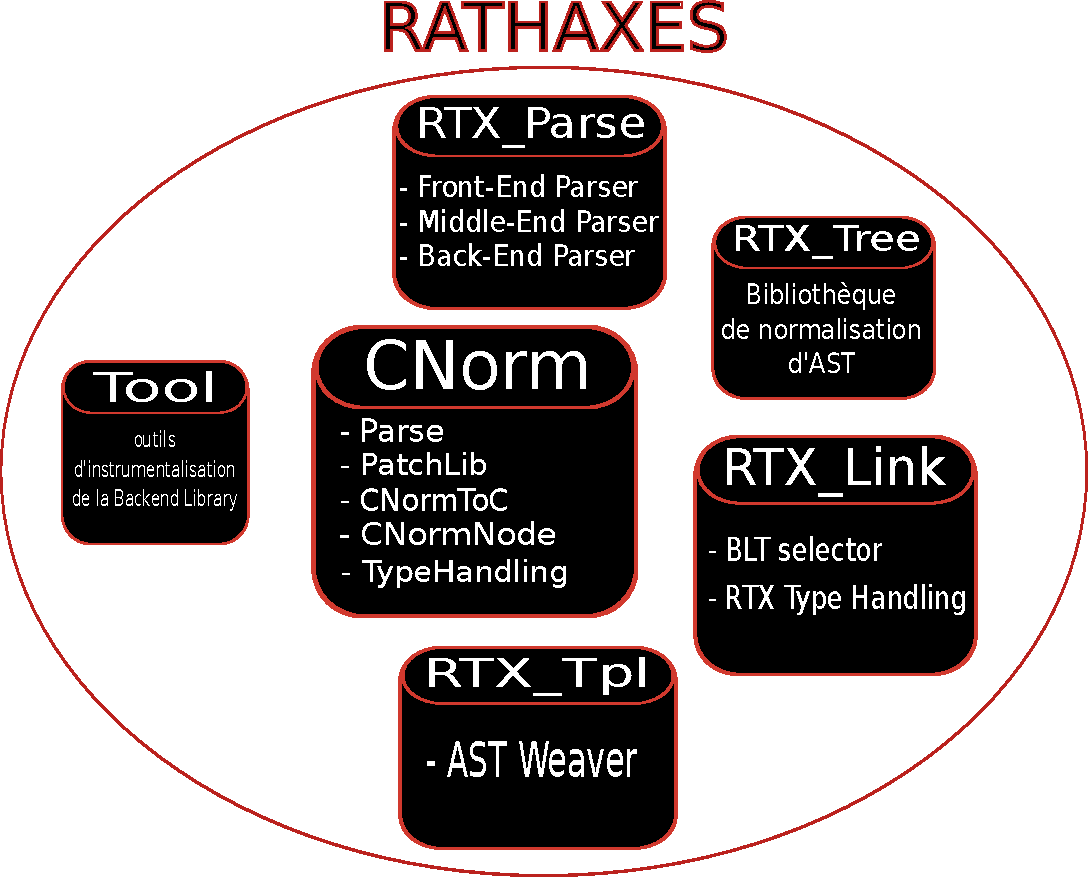
\includegraphics[width=0.95\textwidth]{diagramme_architecture.pdf}

First of all, the \emph{CNorm} library seen previously can be found inside the
compiler. Its role is firstly to generate the final C code, but it also allows
to parse C code. In the case of \rtx, it is overloaded in order to extend
the language and thus to easily parse the templated C code inside the DSL.

The next module, \emph{RTX\_Parse} is the part of the compiler which role is,
as its name implies, to parse the \rtx\ code and built a basic Abstract
Syntax Tree (AST) from it.

\emph{RTX\_Tree} comes with \emph{RTX\_Parse}, as it is a library that helps
normalizing the AST. This way, every type of node in it always respects a given
data representation.

Then, the two modules \emph{RTX\_Link} and \emph{RTX\_Tpl} are the modules that
enter in the process of transforming the raw AST by using the templates in
order to build a complete AST that can be outputted as C code. Their roles will
be detailed in the section \ref{sec:compilationSteps}.

Finally, the \emph{Tool} module, as its name implies, is a series of tools that
offer many kinds of possibilities. For example, a driver on an Unix system
needs a Makefile to be built, a driver on a Windows system need a \texttt{.inf}
file in order to be loaded, \ldots This module offers to generate these kinds
of files.


\section{The different steps of the compilation}
\label{sec:compilationSteps}

From the parsing of a \texttt{.rtx} file to the generation of the driver's C
code, the AST will undergo a number of transformations. However, the interfaces
and the templates of code are also compiled in order to allow caching in the
core of the compiler. That leads to three compilation schemes: an interface's
checking and registration, a template's compilation and a driver's compilation.

\subsection{Steps of an interface's compilation}

The compilation of an interface is a simple task, compared to the two other
parts of the \rtx\ language. We need to validate it, in order to make sure
nothing out of order was written in it (use of an unknown \rtx\ type and
such).

We can identify two steps in the compilation:
\begin{enumerate}
    \item Parsing: construction of an AST normalized by Rtx\_Tree;
    \item TypeChecking: validate the interface against the interfaces it
        depends on (used types, pointcuts and chunks).
\end{enumerate}

Then, the interface is ready for registration and/or installation into the
cache.

\subsection{Steps of a template's compilation}

The compilation of a template can be divided in many steps, since the template
code compilation generates an AST representation and a CodeWorker code that
will help integrate this AST generated from the template into the driver's AST.

We can then identify the following steps:
\begin{enumerate}
    \item Parsing: construction of an AST normalized by CNormNode and
        RTX\_Tree;
    \item Place Holders Identification (Compile): construction of a node
        containing every template placeholder;
    \item Place Holders Parsing (Meta): construction of an AST Node for each
        place holder;
    \item Identification of the \rtx\ types (TypeHash) : indexation of the
        \rtx\ variables \rtx\ used in the code ;
    \item Identification of the local variables (Introspect) : indexation
        of the variables of the target langage for use in the placeHolders;
    \item Type Checking (TypeCheck) : validation of the types against the
        available interfaces from the cache;
    \item Code Generation (Gen): generation of CodeWorker code that resolves
        the linkage of the main AST with the template AST Node.
\end{enumerate}

Afterwards, the developer will be able to install the template into the
Back-End Library. Installing it means that an entry will be added into a
specific cache/registry of the compiler, that helps it associate the right
templates to a given driver at compile-time.


\subsection{Steps of a driver's compilation}
\label{sec:driverCompilation}

The compilation of a driver is a complex process, where every single part of
the DSL is taken in account.

Here is a short list of the steps of its compilation:
\begin{enumerate}
    \item Parsing: construction of an AST from the Front-End syntax;
    \item Type Checking: check of the types used in the Front-End against the
        types described in the Middle-End for validation;
    \item Template selection: the RTX\_Link module selects in the cache which
        templates to load for possible use by checking with the configuration
        variables;
    \item Template instantiation: the RTX\_Tpl module instantiates each
        template AST Node referenced by a Front-End AST Node, and calls the
        linkage resolver functions generated for the template AST Node.
    \item C Code Generation: Generation of the C code from the transformed
        AST;
    \item Utils Generation: the Tool module generates utility files like
        Makefiles for Unix or info files (\texttt{.inf}) for Windows modules,
        \ldots
\end{enumerate}


\subsection{General compilation process}

As you may have already understood, if we talked about three different parts of
the DSL, that means that it is one and only one language. Actually, one could
write a driver with the three parts in one same file. Although this is not
planned to be offered to driver or kernel developers, since their roles are
confined to one part of the language each, it is a possibility. The keywords in
the file will then tell which kind of compilation to activate.

Here is a schema picturing this general process:

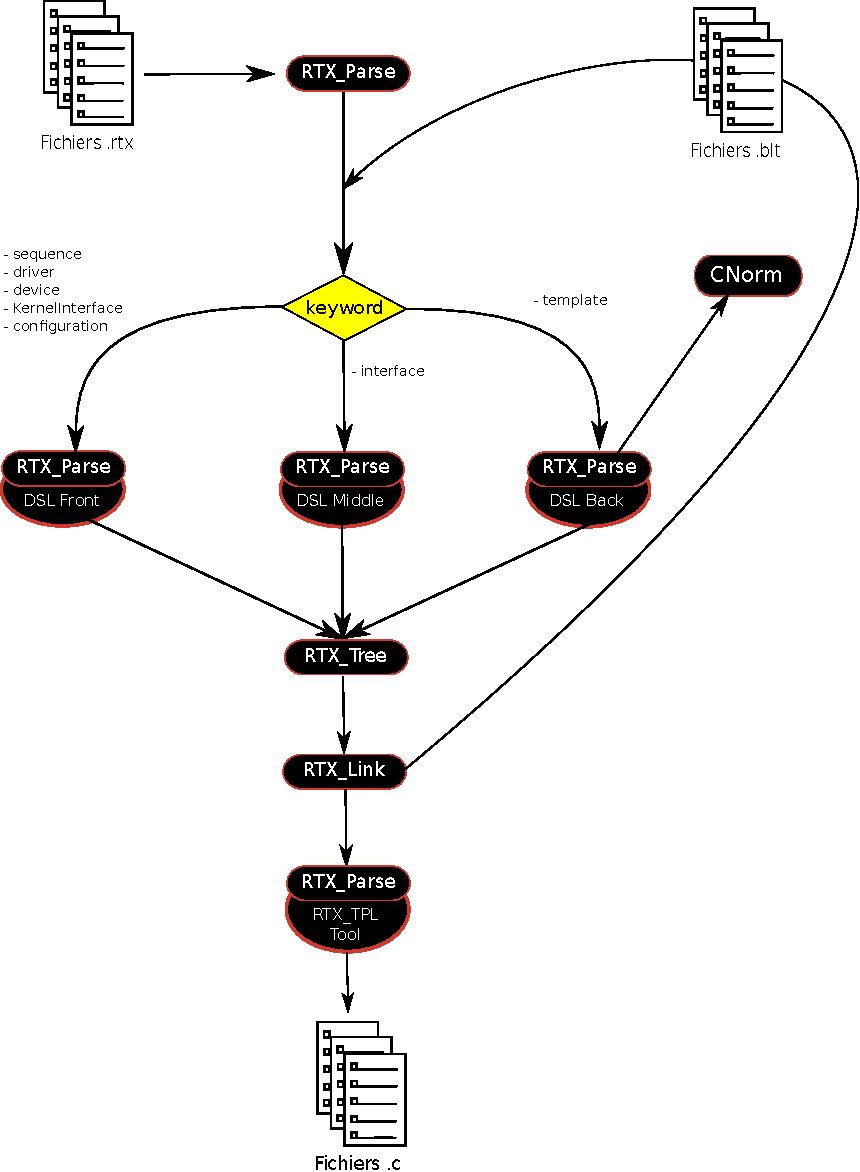
\includegraphics[width=0.95\textwidth]{logigramme.pdf}



\chapter{Details of implementation}


\section{Cache of registered items}

One of the most important and core elements of the compiler is the
\emph{cache}.  Through it, the compiler will be able to keep a list of
registered interfaces and templates that will help finding the right ones to be
used for a driver's compilation and generation.

CodeWorker uses a global variable called ``this'', where one can keep any
information one wants. It is actually used by rathaxes to host the
\emph{cache}. It contains five types of informations:
\begin{enumerate}
    \item Registered interfaces
    \item Registered ``global codes''
    \item Registered templates
    \item Registered chunks
    \item Differential session
\end{enumerate}

Each one of those categories is translated as an item contained in the
``session'' node of the ``this'' tree of CodeWorker. We will call this the
cache session.

Any registered item is a code that has already been compiled and checked by the
compiler, before being added to the cache. Therefore, each of them is
associated to a script file, containing the CodeWorker script that will resolve
the placeholders contained by the code, and a tree file containing the AST of
the code. Those two fields may be optional for some registered items.

Now, we will describe in a more detailed fashion each of those types of items,
and explain their use and how they are used.

\subsection{Registered interfaces}

An interface is a piece of code that enforces the semantic of a sub-system in
\rtx\. In order to avoid inconsistencies throughout the implementation of a
driver, either from the back-end or the front-end, and to prevent the need of
re-parsing each interface at each compilation, each interfaces can be
registered in the cache.

An interface is identified by its name in the cache, and only one interface
associated to an identifier can be registered at the same time. At driver
generation time, or at template compilation time, it is used to check wether
the code implemented matches with the required semantics described by
the interface.

When an interface is stored in the cache, it is an element in an associative
table, which key is the interface's name:
\begin{itemize}
    \item ``.name'': the name of the interface
    \item ``.tree\_file'': the path to the file containing the tree to load
        (Mandatory)
    \item ``.extensions'': list of extensions for this interface, each
        containing:
        \begin{itemize}
            \item ``.with'': the configuration constraint associated to the
                extension
            \item ``.tree\_file'': the path to the file containing the tree
                to load (Mandatory)
        \end{itemize}
\end{itemize}


\subsection{Registered Global code}

A global code is a specific bit of code inside of rathaxes: it's a sort of
chunk outside of a template, that is automatically selected and instantiated as
soon as the associated interface is selected for use. This code is contained
inside a \emph{with} block.

Only one item can be loaded for a given interface. At driver generation time,
each global code associated to each interface will be automatically loaded and
instanciated, as soon as the associated interface is selected by the driver.

When it is registered inside the cache, each global code is inserted as an item
in a list, containing three fields:
\begin{itemize}
    \item ``.with'': the configuration constraint associated (incidentally also
            tells which interfaces it is associated with)
    \item ``.script\_file'': Mandatory
    \item ``.tree\_file'': Mandatory
\end{itemize}


\subsection{Registered Template}

The registered templates are stored in the ``.templates'' field of the cache
session. This field is actually a map where the key is a hash of the template's
prototype, which allows keeping multiple codes for a same template, and where
the value is a list of node describing each registered template. This list
contains unique templates: there can not be two templates with the same
configuration constraint node.

Each registered template's node contains the following fields:
\begin{itemize}
    \item ``.with'': the configuration constraints node for the template
    \item ``.rtype'': the full rathaxes type node of the template
    \item ``.chunks'': a list of items describing the chunks contained by the
            template.
    \item ``.script\_file'': Optional, present only if the template describes
            a type
    \item ``.tree\_file'': Optional, present only if the template describes
            a type
\end{itemize}

Each item in the ``.chunks'' field is actually a way to indicate where the
chunk is stored inside the cache: the key is the fully qualified name of the
pointcut associated, and the value is the index of the chunk inside the list of
chunks associated to the given pointcut. More informations about it will be
given in the description of the registered chunks.


\subsection{Registered Chunk}

The registered chunks are stored inside the ``.chunks'' field of the cache
session. This field is actually a map where the key is the fully qualified name
of the pointcut it is associated to (i.e. interface::name or ::name if not
associated to any interface), and where the value is the list of the chunks
associated to it. This list contains unique chunks : there can not be two
chunks for the same template and the same configuration constraint node.

Each registered chunk contains the following fields:
\begin{itemize}
    \item ``.with'': the configuration constraints node for the template
    \item ``.name'': the fully qualified name of the pointcut
    \item ``.tpl\_id'': the hash of the containing template
    \item ``.script\_file'': Mandatory
    \item ``.tree\_file'': Mandatory
\end{itemize}


\subsection{Differential session}

What we call the ``Differential session'' is actually a sort of register of
every modification applied over the cache during the compilation process. This
allows rolling back the unwanted operations before saving the cache, in order
to avoid any inconsistency. This also allow the "install" operation to take
place.

The differential session is stored inside the ``.temp'' field of the cache
session, and it structured the same way the cache session is. Each one of its
registered nodes are actually references to the nodes added to the cache
session. This is how they can be easily removed.

When the cache is validated, the compiler, depending on its command-line
arguments may install the new compiled files into the persistent cache. The
process of installing consists of three operations:
\begin{itemize}
    \item Computing a file name from informations about the registered item
    \item Copying the pre-compiled files into the backend library
    \item Updating the files paths into the cache
\end{itemize}

Thanks to the temporary session, those operations can be easily managed, and
the cache can stay consistent.


\subsection{Cache API}

In this section, we will describe every ``public'' function of the cache, in
order to make maintaining the cache's code easy. Each one of these functions is
coded in the file rtxLink.inc.cws of the compiler's scripts.

There are mainly two use cases for the cache. The first use-case is to fill it
with a file being compiled. The second is to use it in order to load the script
and tree file for a place holder resolution, meaning a code generation.

\vspace{20pt}

The functions to be used in both of those use cases are the following.

\begin{lstlisting}
function rtxLink_LoadCache();
\end{lstlisting}
The function \emph{rtxLink\_LoadCache} is used to load the cache's information
tree from the file located in the backend library directory. If this function
is not called before calling another function of the cache, it will be
considered as an empty cache, and may overwrite the old one if saved.

\begin{lstlisting}
function rtxLink_SaveCache();
\end{lstlisting}
The function \emph{rtxLink\_SaveCache} is used to save the cache's state into
the backend library directory. If there was any change made to the cache, this
function will automatically save the generated files into the backend library
directory.

\begin{lstlisting}
function hashTemplatePrototype(theRType     : node,
                               out_ref_hash : reference);
\end{lstlisting}
The function \emph{hashTemplatePrototype} takes a rtype node as a first
argument.  This node describes a template's type (identified by its name and
parameter types). The second argument is a reference used to return the hashed
prototype.  This function is used throughout the code in order to get a string
identifying a template.

\vspace{20pt}

The following functions are used in order to fill the cache.

\begin{lstlisting}
function rtxLink_RegisterToCache(local_node : node);
\end{lstlisting}
The function \emph{rtxLink\_RegisterToCache} walks through a rathaxes AST and
registers each of its with blocks, templates and chunks into the cache session.

\vspace{20pt}

The following functions are used to manipulate the cache in order to resolve
place holders and generate code. We can then identify three use cases:
resolving a pointcut (meaning selecting AND instanciating every chunk
associated to it), resolving a global code instanciation, resolving a chunk
through the associated template and finally resolving a template type mapping.

\begin{lstlisting}
function rtxLink_findGlobalCode(with_values  : node,
                                out_code_ref : reference);
\end{lstlisting}
The function \emph{rtxLink\_findGlobalCode} retrieves the global code node
matching the configuration given through the with\_values argument, and returns
it through the reference out\_code\_ref.

\vspace{20pt}

Functions used to resolve a template (or one of its chunks):
\begin{lstlisting}
function rtxLink_findTemplates(theRtype : node,
                               out_tpls : node);
\end{lstlisting}
The function \emph{rtxLink\_findTemplates} retrieves the full list of templates
matching the type describing node theRtype. It then copies the whole list into
the out\_tpls parameter.

\begin{lstlisting}
function rtxLink_selectUniqueTemplate(templates : reference,
                                      config : node);
\end{lstlisting}
The function \emph{rtxLink\_selecteUniqueTemplate} selects one template (the
one whose configuration constraints match the most the configuration given in
the config parameter) from a list of templates. The argument templates must be
a list of templates retrieved through the function
\emph{rtxLink\_findTemplates}. The selected template is then set into the
``templates'' parameter. In the case of a type mapping resolution, the node
retrieved in the ``templates'' argument can be directly given to the
\emph{rtxLink\_LoadScript} function.

\begin{lstlisting}
function rtxLink_selectChunkFromTemplate(theTemplate : node,
                                         chunkName : value,
                                         theChunk : reference);
\end{lstlisting}
The function \emph{rtxLink\_selectChunkFromTemplate} takes a template node
retrieved through the \emph{rtxLink\_selectUniqueTemplate} function, and a
chunk name (fully qualified name, i.e. "interface::name"). Then, it sets the
reference ``theChunk'' to the chunk associated with the template if it could be
found. In case of failure, the function returns false. This function is used
when one wants to resolve a given chunk from a precise template. This is the
case for internal functions of the compiler, and for some template type
resolutions.

\vspace{20pt}

Functions used to resolve a pointcut:
\begin{lstlisting}
function rtxLink_findChunks(pointcut_name : node,
                            out_chunks : node);
\end{lstlisting}
The function \emph{rtxLink\_findChunks} retrieves a list of chunks associated
to a given pointcut name. The list is copied into the ``out\_chunks''
parameter.


\begin{lstlisting}
function rtxLink_selectCompatibleChunks(chunks : node,
                                        config : node);
\end{lstlisting} The function \emph{rtxLink\_selectCompatibleChunks}works on a
list of chunks retrieved through the function \emph{rtxLink\_findChunks}, and
keeps only the chunks matching the configuration given through the ``config''
parameter. From here on, one can give each of the chunks to the function
\emph{rtxLink\_LoadScript} for the code generation.


\begin{lstlisting}
function rtxLink_LoadScript(cache_node : node,
                            out_ref_tree : reference);
\end{lstlisting}
The function rtxLink\_LoadScript loads the script and the tree (into the
reference given) associated to the cache node. It prevents silently double
loading of a script, and needs to be given a node from within the cache
matching either a chunk, a template or a global code. The cache node can be
obtained through the latter previously described functions.



%\section{Interface compilation}

%
% TODO
%

\section{Template compilation}

In \rtx, two kinds of templates exist. Those are the sequence templates and the
type templates. Both share common passes for their compilation, though there
are some differences between them.

Each pass of the templates compilation is coded inside the matching file in the
directory named ``rtxTpl'' in the compiler's script directory. We can currently
identify the following passes in order:
\begin{enumerate}
    \item Parse: \texttt{rtxParse/rtxBack.inc.cws};
    \item Compile: \texttt{rtxTpl/rtxCompile.inc.cws};
    \item Meta: \texttt{rtxTpl/rtxMeta.inc.cws};
    \item TypeHash: \texttt{rtxTpl/rtxTypeHash.inc.cws};
    \item Introspect: \texttt{rtxTpl/rtxIntrospect.inc.cws};
    \item TypeCheck: \texttt{rtxInterfaces/rtxInterfaces.inc.cws};
    \item Gen: \texttt{rtxTpl/rtxGen.inc.cws}.
\end{enumerate}

Many of those passes could have been done in one walk through the AST, but for
maintenance purposes, we chose to separate them. In terms of code, each pass in
the compiler is made with a templated \emph{CodeWorker} function, which is
specialized on the type of the node walked through. This allows specializations
that help walking through the different types of nodes. For example, a node
containing a list of elements could loop over the elements it contains, while a
node containing two specific fields could only walk through those fields. By
the way, This allows a specific management of the meaningful nodes for each
pass. Here is the description of the passes that are applied over the tree for
a template's compilation process.

\subsection{Parse}

This is the common pass for every compilation process throughout \rtx\'s
compiler. Every parsing code can be found inside the directory rtxParse/ of the
compiler's scripts. The common necessities can be found in the file
rtxCommon.inc.cwp and the templates-only rules can be found inside the file
rtxBack.inc.cwp. The parsing pass builds an AST standardized with the help of
the rtxNode module.

\subsection{Compile}

This pass has for objective to identify every single bit of code that is
instrumented code: the \emph{placeholders}. Each \emph{placeholder}
identified is then added into a field named ``.compile'' into the
instrumented C root block. This field is a list of \emph{placeholders},
associated with information to help find its real place inside the tree.

\subsection{Meta}

This pass walks over every single \emph{placeholder} identified during the
previous pass. Each placeholder is then parsed independently from its context,
and the resulting node is added into the current \emph{placeholder}'s node.
This newly created node will be used later for the final code generation, to
resolve the \emph{placeholder}.

\subsection{TypeHash}

This pass tries to identify every \rtx\ variable declaration, in order to store
both the variable name and its actual type inside a specific node named
``.type\_map'', for each instrumented code block (or \emph{chunk}). This allows
referring to the \rtx\ variables in the \emph{placeholder} syntax, and checking
their validity. This is then used for the \emph{placeholder} resolution.

\subsection{Introspect}

After the \rtx\ types were all identified and extracted during the previous
pass, this one tries to identify every instrumented code variable declaration
to associate the types (be it a \rtx\ type or a base code type) with the
variables. This helps the \emph{placeholder} resolution mechanism when we are
trying to use a local variable.

\subsection{TypeCheck}

Once the code is properly processed, and ready to generate some code, we can
check the \emph{template}'s implementation against the contract expressed in
the form of one or more interfaces. Then, for each encountered \rtx\ type or
prototype (template's prototype), the compiler checks it against the ones
described in the interface. This causes the compilation process to halt in
case of failure, after trying to check every checkable bit of code. Thus,
every use of a \rtx\ type, every template prototype, every pointcut, every
chunk is checked for existence (if it was never described, it is an error),
and for validity (present in an interface the template depends on, or
explicitly called).


\subsection{Gen}

The last thing to do before registering a template into the compiler's cache is
to generate the \emph{CodeWorker} script that will resolve every
\emph{placeholder} of every block of instrumented code. This is the code that
will be called in order to resolve the \emph{placeholders} and therefore obtain
a fine AST to weave into the caller template's. The code generated
depends on the type of the \emph{placeholder}. It won't be the same if the
\emph{placeholder} is a declaration of a variable of \rtx\ type, or a
\emph{pointcut}. Each chunk is then associated to a generated templated
\emph{CodeWorker} function, which contains the calls to resolve each
one of its \emph{placeholders}.

\subsection{Type templates specificities}

The compilation process is the same for type templates and sequence templates.
The only difference is that type templates contain a \emph{map} block,
which describes the mapping to be made available for use when using a variable
of this type.

Therefore, a templated \emph{CodeWorker} function is generated for the
template's mapping, in the same way a function is generated for each chunk it
contains. This function manages every mapping associated to the template and
resolves each one of them. See the code generating function in the file
\texttt{rtxTpl/rtxGen.inc.cws}, called
``\texttt{gencodeworker<"\_\_rtx\_tpl\_type\_map\_\_">}''.

\section{Driver compilation}

The compilation of the driver (with the front-end description) is one of the
most sensible parts of the whole compilation process in \rtx\. It uses both
others parts of the language.

Each compilation pass is written in a separate file, and the scripts can be
found in the compiler's scripts directory. We can currently identify the
following passes and their containing files:
\begin{enumerate}
    \item Parse: \texttt{rtxParse/rtxFront.cwp}
    \item TypeCheck: \texttt{rtxInterfaces/rtxInterfaces.inc.cws}
    \item Configuration Building: \texttt{rtxFront/rtxTools.inc.cws,
                                          rtxNode/rtxNode.inc.cws}
    \item Generation: \texttt{rtxFront/rtxGenerate.inc.cws,
                              rtxTpl/rtxResolve.inc.cws}
\end{enumerate}

In the same way as the template compilation passes, many of the passes are
coded into CodeWorker templated functions, in order to ease the walking of
the AST, and to specialize only for the nodes that are relevant for the task.
We will now describe each step.

\subsection{Parse}

This is the common pass for every compilation process throughout \rtx\'s
compiler. Every parsing code can be found inside the directory rtxParse/ of the
compiler's scripts. The common necessities can be found in the file
rtxCommon.inc.cwp and the templates-only rules can be found inside the file
rtxBack.inc.cwp. The parsing pass builds an AST standardized with the help of
the rtxNode module.

\subsection{TypeCheck}

The TypeCheck pass for the front-end has two main parts: first, the check
against the interfaces, and second the consistency check.

First, we check that the interfaces given in the driver block description
describe properly what we are using:
\begin{itemize}
    \item the implementation prototype: we check that every templated which
        algorithm is written in the driver is either required (implementation
        is mandatory), or optional. No ``provided'' should ever find its way
        into the front-end implementation, those being reserved for use by
        calls from either the front-end or the back-end
    \item the code of the implementation: analyzed in order to check whether
        the sequences and types used are provided or not, since those are the
        the only ones that should be usable in a chunk of \rtx\ code.
    \item the configuration block: each variable expected must be described in the associated interface(s).
\end{itemize}

When the checks about the interfaces (depending on the interfaces written
in the dependency list of the front-end) are done, consistency checks are
run against the front-end itself. For instance, the registers'description
is checked in order to prevent the values written to be incompatible with the
bit mask written in the "LIKE" statement.

The checks done, we can now go on to prepare the generation.

\subsection{Configuration Building}

The configuration building step is as its name implies. The configuration block
is stored in an AST but its form is not easily usable for the selection process
of the templates for the generation. We need to translate it into an usable
data structure. The associated file does the job, and generates the multiple
configurations described in the block (each extension depending on a
configuration value creates a branch in the possible configuration schemas).

\subsection{Generation}

Finally, the front-end AST is prepared for the generation process. This pass
may be one of the most complex of the \rtx\ compiler. Actually, all it does is
iterate on the available configurations, and start the generation for each one.

For each generation, the driver block is retrieve, and the template resolution
is started, with the global code as a root.

Warning: Currently, there is no pre-selection of the used templates for the
resolution of the C code, and thus every single matching chunk
(configuration-wise and template-wise) is inserted into their associated
pointcut.

The resolution is recursive, and for each placeHolder encountered, a resolver
function is called, which instanciates the AST part, and resolves it before
inserting it in-place of the original placeHolder. This may seem simple but
is permitted by the multiple steps done in each compilation process for
each part of the \rtx\ language.

%
% TODO
%




\end{document}
